\documentclass[conference]{IEEEtran}
\IEEEoverridecommandlockouts
% The preceding line is only needed to identify funding in the first footnote. If that is unneeded, please comment it out.
%Template version as of 6/27/2024

%tommaso
\usepackage[utf8]{inputenc}
\let\Bbbk\relax
\usepackage{newtxtext,newtxmath}
\usepackage{float}
\usepackage{booktabs}
\usepackage{makecell}
\usepackage{hyperref}
\usepackage[backend=biber,style=numeric]{biblatex}
\addbibresource{resources/bibliography.bib}
%\usepackage{cite}
%end tommaso
\usepackage{amsmath,amssymb,amsfonts}
\usepackage{algorithmic}
\usepackage{graphicx}
\usepackage{textcomp}
\usepackage{xcolor}
\def\BibTeX{{\rm B\kern-.05em{\sc i\kern-.025em b}\kern-.08em
    T\kern-.1667em\lower.7ex\hbox{E}\kern-.125emX}}
\begin{document}

\title{Complex Network Exploration and Analysis: Epinions Dataset}

\author{\IEEEauthorblockN{Tommaso Tragno}
\IEEEauthorblockA{\textit{Faculdade de Ciências} \\
\textit{Universidade de Lisboa}\\
Lisboa, Portugal \\
fc64699@alunos.fc.ul.pt}
\and
\IEEEauthorblockN{Antonio Alampi}
\IEEEauthorblockA{\textit{Faculdade de Ciências} \\
\textit{Universidade de Lisboa}\\
Lisboa, Portugal \\
fc64316@alunos.fc.ul.pt}
\and
\IEEEauthorblockN{Meike van der Veen}
\IEEEauthorblockA{\textit{Faculdade de Ciências} \\
\textit{Universidade de Lisboa}\\
Lisboa, Portugal \\
fc66408@alunos.fc.ul.pt}
}

\maketitle

\begin{abstract}
This report examines the "soc-Epinions1" dataset, a who-trusts-whom social network, to explore trust dynamics and network structure. A core subset (30\% of original dataset) was created through recursively removing nodes with a degree of 4 or lower for detailed analysis, focusing on influential nodes and community structures. A basic analysis was performed on the full dataset and a more detailed analysis including community detection and information flow simulation on the core subset. Key findings reveal the dataset's scale-free properties with tightly knit communities and asymmetry in trust relationships. Through the Louvain analysis, communities for both the full dataset and the subset with a medium modularity were found, with a value that was slightly higher for the full dataset than for the subset. For both the full dataset and core subset, the majority of the nodes was in the 10 largest communities and 10 largest hubs were a member of the three largest communities found in the core subset. Hubs play a critical role in information propagation, as demonstrated through simulation of opinion dynamics. These insights provide real-world applications for reputation systems, targeted marketing, and influence optimization. 
\end{abstract}

\begin{IEEEkeywords}
Epinions,
Who-trusts-whom Networks,
Social Network Analysis,
Community Detection,
Spectral Clustering,
Opinion Dynamics.
\end{IEEEkeywords}

\section{Introduction}
This report presents an exploration and analysis of the "soc-Epinions1" dataset, obtained from the Stanford Large Network Dataset Collection (SNAP). This dataset represents  a who-trusts-whom online social network derived from Epinions.com (now known as Shopping.com). On this platform, users could establish trust relationships with one another, forming a Web of Trust. The platform used this web of trust in combination with review ratings to determine which reviews were displayed to users.
The analysis began with a descriptive study of the dataset, followed by an examination of a representative subset to conduct a more detailed analysis. 

The repository containing the code for the analysis could be found by clicking this
\href{https://github.com/tratom/fcul-cda-project}{Project Repository Link} ,
or going to the next url: \url{https://github.com/tratom/fcul-cda-project}

\subsection{The Dataset}
\subsubsection{SNAP Statistics}
The "soc-Epinions1" dataset consists of the following characteristics, as documented on the SNAP platform and confirmed by our study:

\begin{table}[h!]
\centering
\begin{tabular}{|c|c|}
\toprule
\textbf{Nodes (users)} & 75,879 \\
\textbf{Edges (trust relationships)} & 508,837 \\
\textbf{Nodes in the largest WCC} & 75,877 (1.000) \\
\textbf{Edges in the largest WCC} & 508,836 (1.000) \\
\textbf{Nodes in the largest SCC} & 32,223 (0.425) \\
\textbf{Edges in the largest SCC} & 44,3506 (0.872) \\
\textbf{Average Clustering Coefficient} & 0.1378 \\
\textbf{Number of triangles} & 1,624,481 \\
\textbf{Fraction of closed triangles} & 0.0229 \\
\textbf{Network Diameter} & 14 \\
\textbf{90-percentile effective diameter} & 5\\
\bottomrule
\end{tabular}
\caption{SNAP Statistics for Epinions dataset.}
\label{tab:network_stats}
\end{table}

\subsection{Literature Review}
The Epinions dataset was introduced by Richardson et al. (2003)\cite{richardson2003trust} in Trust Management for the Semantic Web. In their paper, they study methods for computing personalized sets of trusts for users of the Semantic Web, which they test on the Epinions dataset. They suggest approaches which given a number of users that a user explicitly trusts, computes trust values for all other users in the network, giving the user a subjective recommendation of the trustworthiness of information sources. 
Since then, the Epinions dataset has been used in many studies on different topics related to (social) networks and trust. De Meo et al.(2014)\cite{de2014trust} for example studied the role of trust in group formation and evolution in social networks and argue that compactness of networks should consider the mutual trustworthiness between group members besides their similarities. Golzardi et al.(2023)\cite{golzardi2023trtcd} explore the prediction of trust routes between users in social networks. 

The Epinions dataset has also been used to test community detection algorithms. Leskovec et al.(2008)\cite{leskovec2008dynamics} for example introduced a novel way of clustering large social networks, using Epinions as one of many datasets. They found that large networks have very different community structures compared to small networks. Another area in which the Epinions dataset has been valuable is in understanding the spread of for instance opinions, beliefs and behaviours within social networks. This was for example the topic of the study by Como et al. (2016)\cite{como2016threshold}, which uses the Threshold Model of cascades on the Epinions network to simulate these dynamics. 
In recent years, the Epinions dataset has been increasingly used in research on recommender systems, which have become increasingly important on online platforms for suggesting items based on user preferences. Liu et al.(2019) \cite{liu2020collaborative} developed a collaborative filtering recommendation algorithm that incorporates multiple relationships in social networks. Atdag and Bingol(2019) \cite{atdag2021computational} also used the Epinions dataset to design models for commercial advertisements, focusing on how to maximize ad reach and user engagement through trust-based connections. Nzeko'o et al. (2024) \cite{nzeko2024time} propose strategies that consider both the timing and content of users interactions to better estimate implicit trust. 
The Epinions dataset has thus been used in advancing research on trust, community structure, opinion formation, and recommender systems. As more studies continue to use the dataset for doing research in these areas, the dataset remains a key resource for understanding how trust operates in social networks and how this impacts various applications.

\subsection{Aim of the Study}
In this report, the Epinions data set will also be analysed to gain more insight into the structure of and communities in who-trusts-whom networks, as well as the spread of opinions through such a network. A basic analysis of the full subset will be performed and a subset will be created on which the detailed analysis will be carried out. This will be done t reduce computational power and to compare the subset to the full dataset. 

\section{Methodology}

In this study, a detailed analysis will be performed on a subset of the Epinions dataset. We will perform a basic analysis of both the full dataset and the subset, to provide insight into the properties of the dataset and later compare the statistics with the properties of the subset. This way, we can also gain some insight into the robustness of the dataset. In the sections below, the process and justification for creating the subset and the methods for carrying out the analyses will be explained. 

\subsection{Subset Creation}
There are different methods that can be used to select a subset from the full dataset. Since the aim of our study is to gain more insight into the trust dynamics in the network by analysing the characteristics and dynamics of the subset, our goal was to include the nodes that are most important and influential for these dynamics. Customers that only trust a few other customers contribute less to the trust dynamics and removing them will have the least impact on the generation of meaningful results. Therefore, the detailed network analysis was performed on the “core” of the network. 

\subsubsection{Core network subset}
The “core” of the network was created by recursively removing the nodes with a total degree below a certain threshold, until no more nodes were removed. To obtain a graph with approximately 30\% of the initial nodes, a threshold equal to 4 (sum of in-degree + out-degree) was set. In this way, a subset is created that is significantly smaller than the full dataset, which offers computational advantages, while only losing nodes that are relatively insignificant in the dynamics of the web of trust. The resulting core graph has 23,503 nodes and 431,564 edges. Below there is a plot of the core network.

\begin{figure}[H]
    \centerline{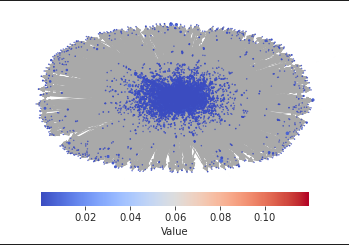
\includegraphics[width=0.4\textwidth]{img/core_network.png}}
    \centering
    \caption{Core network plot.}
    \label{fig:core_network_plot}
\end{figure}

\subsubsection{Reversed Graph}
The reverse graph was also created. It flips the direction of all edges of the core graph, making it represent "who is trusted by whom" rather than "who trusts whom". This makes it easy to identify users who are highly trusted by many others and analyze their influence within the network. The descriptive statistics of the reverse graph will be the same as those of the core graph, also the plot of log-log out-degree distribution and log-log in-degree distribution are the same. The obvious result to expect is that what were previously the top 5 in-degree nodes of the core graph will now be the top 5 out-degree nodes of the reverse graph, and vice versa. Subsequently it will be used to depict how the subgraphs centered in a node vary, and to perform simulation. Below there is a plot of the reversed graph.

\begin{figure}[H]
    \centerline{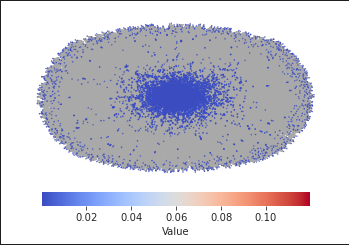
\includegraphics[width=0.4\textwidth]{img/reversed_core_network.png}}
    \centering
    \caption{Reverse core network plot.}
    \label{fig:reverse_core_network_plot}
\end{figure}

\subsection{Basic analysis}
\subsubsection{Data Loading and Preprocessing}
The dataset was imported as a directed graph by loading its edge list. We used the \textbf{NetworkX} python library for all network computations and analysis.

\subsubsection{Statistics}
For the full dataset we computed the statistics to compare them to the ones reported on SNAP, getting the same values for all except average clustering coefficient, triangles and diameter. About the discrepancy in the \textbf{average clustering coefficient and triangles} calculated in our study, this suggests potential methodological differences or updates in computation. It was also not possible to calculate the length of the diameter, as the direct graph is not strongly connected, and would also be unconnected if it were to be converted to an indirect graph.  Besides this, the 90th percentile effective diameter could not be computed because, for large graphs, this approach is computationally expensive due to shortest path calculation for all pairs which is required. Therefore, for the subset the same statistics were computed as for the full dataset, except for the 90th percentile effective diameter.

\subsubsection{Degree centrality and distribution analysis}
Additional metrics related to the degree centrality as well as the log log degree distribution were computed for both the full dataset and subset to gain insight into the structure of the network and the most important nodes. The 10 nodes with the highest in- degree, highest out-degree and highest total degree were obtained. These parameters indicate the hubs of the network, which were also analyzed more closely via a hub analysis. Hub analysis was carried out to look for the presence of hubs within our dataset, i.e. nodes with high degree, both in-degree and out-degree. Hub nodes are nodes that play a crucial role in the network by having a nodes with a high number of connections or strong influence on the network's structure and dynamics.
Degree Centrality measures the proportion of nodes a given node is directly connected to. It is normalized by dividing the degree of the node by \(N-1\), where N is the total number of nodes in the graph.
To get more information about the centrality of all the nodes, the mean and median degree and mean and mean degree centrality were computed. In addition, the log-log degree distribution was generated, through creating a scatter plot with the degrees on the x-axis and the number of nodes that have that number of degrees on the y-axis. Both axes are scaled logarithmically to identify a power-law distribution, in which the relationship between the degree k of a node and its probability \(P(k)\) follows the equation: \[P(k) \sim k^{-\alpha}\]
This relationships results in a straight line with slope -$\alpha$ on a log-log plot. This straight line indicates a scale-free network, in which most nodes have a small number of connections, while a few nodes have disproportionally high numbers of connections. The steeper the line, the more strongly this phenomenon is present. 

\subsection{Detailed analysis of the subset}
To gain more insight into the structure, we have applied community detection algorithms to the core network. We have used Louvain for community detection and K-means for spectral clustering. In addition, we have simulated the flow of information through the network to gain insight into how this happens. We elaborate on these more detailed analyses in the sections below.

\subsubsection{Louvain Community Detection}
The Louvain algorithm was used to detect communities in both the full dataset and core network, to compare the results. The communities of the core network were further analysed. The Louvain algorithm was developed by Blondel et al.(2008) \cite{blondel2008fast} and is able to handle large networks efficiently. The algorithm first places all nodes in their own community and then iteratively reassigns each node into the community of its neighbor if this increases the modularity. In the next phase, the algorithm does the same, only now it moves the communities from the first steps into the neighboring community if it increases modularity. It keeps repeating these phases until no further improvements in modularity can be made. The algorithm as used in \cite{blondel2008fast} is designed for undirected networks. Therefore, an adjusted algorithm using the directed modularity of Arenas et al. (2007) \cite{arenas2007size} was used, which was developed by Dugue and Perez (2022) \cite{dugue2022direction}. They found that using directed modularity is more efficient in the case of directed graphs. The algorithm was developed for C++, but this was the only Louvain algorithm we were able to find that was adjusted for directed graphs and the python binding unfortunately did not work. Therefore this part of the code is in C++. 

The communities of the core network were analyzed by evaluating the community sizes, the intra-community and inter-community dynamics edges of the largest communities and the communities assignment of the hubs in the network. 


\subsubsection{Spectral Clustering Analysis}
The goal of this analysis was to partition the core graph into meaningful clusters using spectral clustering techniques. This involved computing the Laplacian matrix, which was derived from the graph's adjacency and degree matrices, identifying spectral gaps in eigenvalues to determine the optimal number of clusters, and performing k-means clustering. The clustering results were then analyzed in terms of cluster sizes, density, and modularity contribution. 
To determine the optimal number of clusters, a spectral gap analysis was conducted. By examining the eigenvalues, significant gaps were identified, and the value k=9 was selected as the number of clusters. This choice was guided by the largest spectral gaps observed, which indicated separations in the graph's structure suitable for clustering.
Following the determination of k, the k-means algorithm was applied to the eigenvectors associated with the nine smallest eigenvalues. The first eigenvalue, corresponding to the trivial zero eigenvalue, was excluded from this process. This application of kkk-means allowed the identification of clusters in the graph's lower-dimensional spectral space.
After clustering, the results were carefully analyzed. The clusters were evaluated based on their size and density, the latter being a measure of how closely connected nodes within each cluster were relative to the maximum possible connections. Additionally, the modularity contribution of each cluster was assessed, providing insight into how each cluster contributed to the overall modular structure of the graph. This comprehensive analysis highlighted the meaningful divisions within the graph and the structural significance of each cluster.

\subsubsection{Simulation: Influence of Trusted Nodes on Opinion Dynamics}
This analysis explores how influential nodes (hubs) in a "who trusts whom" network can impact the opinions of nodes that trust them. Specifically, the study investigates how trust relationships propagate influence through the network. To achieve this, we:

\begin{itemize}
    \item Extracted the top 20 hubs from the "who trusts whom" core graph graph, representing nodes that are most trusted by others.
    \item Reversed the graph's direction, transforming it into a "who is trusted by whom" graph, where directed edges point from trusted nodes to the nodes they influence.
    \item Simulated the spread of influence through the reversed graph to understand how the opinions of highly trusted nodes affect the opinions of those who trust them.
\end{itemize}

\paragraph{Simulation Design}

\begin{itemize}
    \item \textbf{State Definitions:}
    \begin{itemize}
        \item \textbf{"Awake" State:} A node has adopted the opinion of an influencer.
        \item \textbf{"Asleep" State:} A node has not yet adopted the opinion.
    \end{itemize}
    \item \textbf{State Transition Rules:}
    \begin{itemize}
        \item Nodes can transition from "asleep" to "awake" if:
        \begin{enumerate}
            \item At least one of their influencers (trusted nodes) is "awake."
            \item With a small probability (Pawaken=0.2P), representing spontaneous adoption.
        \end{enumerate}
    \end{itemize}
    \item \textbf{Stop Condition:} The simulation halts when no nodes change state between consecutive steps or after 100 steps.
\end{itemize}
All nodes are updated simultaneously in each step.
At each step, the number of nodes transitioning from "asleep" to "awake" was recorded to evaluate the propagation dynamics.

\section{Results}
\subsection{Network Statistics}

\begin{table}[h!]
\centering
\begin{tabular}{|c|c|c|}
\toprule
\textbf{Statistic} & \textbf{Full Dataset} & \textbf{Core Dataset (subset)} \\
\midrule
\textbf{Nodes (users)} & 75,879 & 23,503 \\
\textbf{Edges (trust relationships)} & 508,837 & 431,564\\
\textbf{Nodes in the largest WCC} & 75,877 & 23,497\\
\textbf{Edges in the largest WCC} & 508,836 & 431,552 \\
\textbf{Nodes in the largest SCC} & 32,223 & 21,498 \\
\textbf{Edges in the largest SCC} & 44,3506 & 418,634 \\
\textbf{Average Clustering Coefficient} & 0.1102 & 0.2195 \\
\textbf{Number of triangles} & 740,310 & 738,999 \\
\textbf{Network Diameter} & $\infty$ & $\infty$ \\
\textbf{Assortativity Coefficient} & -0.0413 & -0.04544\\
\bottomrule
\end{tabular}
\caption{Computed Statistics for all the dataset.}
\label{tab:computed_stats}
\end{table}

As it can be seen from the table above, the value of the average clustering coefficient between the core graph and the original graph is different. This can be attributed to the structural differences between the two. The clustering coefficient measures how well the neighbors of a node are connected. A high clustering coefficient indicates a tendency for nodes to form tightly-knit groups. So, the core graph, with fewer nodes, is likely composed of more densely connected nodes, and also contains nodes with a degree above a threshold, therefore this could naturally exclude peripheral nodes and isolate regions of higher connectivity. This can naturally lead to a higher clustering coefficient. So, in conclusion it can be said that the original graph's average clustering coefficient indicates a relatively low level of clustering: this is expected in large-scale, sparse networks like social trust networks, on the contrary the core graph's average clustering coefficient is nearly double, suggesting that the core graph is much more densely connected, with a higher prevalence of tightly-knit groups. 

Similar reasons explain why the assortativity coefficient (that measures the tendency of nodes in a network to connect with other nodes that are similar in some property) increases between the full dataset and the core graph.
Finally, about the number of the triangles, nodes were removed during the construction of the core graph, so the triangles they participated in were also removed, reducing the total count in the core graph.

\subsection{Degree Analysis}

\begin{table}[h!]
\centering
\begin{tabular}{|c|c|c|}
\toprule
\textbf{Statistic} & \textbf{Full Dataset} & \textbf{Core/Reverse Dataset} \\
\midrule
\textbf{Mean Degre} & 13.4118 &  36.7242 \\
\textbf{Median Degree} & 2 & 10 \\
\bottomrule
\end{tabular}
\caption{Degree Analysis for all the dataset.}
\label{tab:degree_stats}
\end{table}

These statistics give insights into the degree distribution of the two graphs and how the core subset (or reverse graph) differs from the full graph. The mean degree of 13.411 indicates that, on average, each node in the full graph is connected to approximately 13 nodes. Is a very small value, considering that the graph contains 75879 nodes. On the contrary, the mean degree of 36.724 in the core graph is significantly higher than the full graph’s mean degree. This indicates that the core graph is denser, with nodes having more connections on average. About the median degree, the value of 2 in the graph indicates that more than half of the nodes in the graph have 2 or fewer connections. This suggests that the graph is sparse in the sense that a significant portion of nodes are only loosely connected. The median degree of 10 is also higher in the core graph, meaning that at least half of the nodes in the core graph are more strongly connected than in the full graph. This suggests that the core graph includes higher-degree nodes compared to the full graph.
The core graph has a higher mean degree and median degree than the full graph, which underlines again that the core consists of a more tightly-knit and connected group of nodes

\subsubsection{Degree Distribution}
The graph below shows the log-log in- and out-degree distribution for both the full dataset and the core dataset. 

\begin{figure}[H]
    \centerline{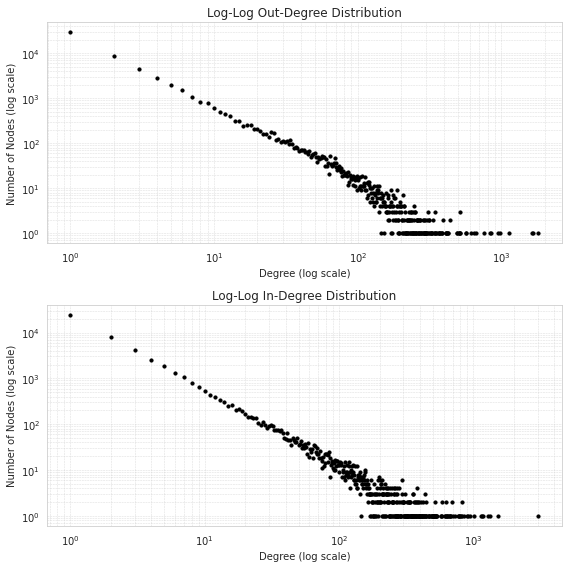
\includegraphics[width=0.4\textwidth]{img/loglog_graph.png}}
    \centering
    \caption{log-log degree distribution for both out- and in-degree for the full dataset}
    \label{fig:log_dataset}
\end{figure}

\begin{figure}[H]
    \centerline{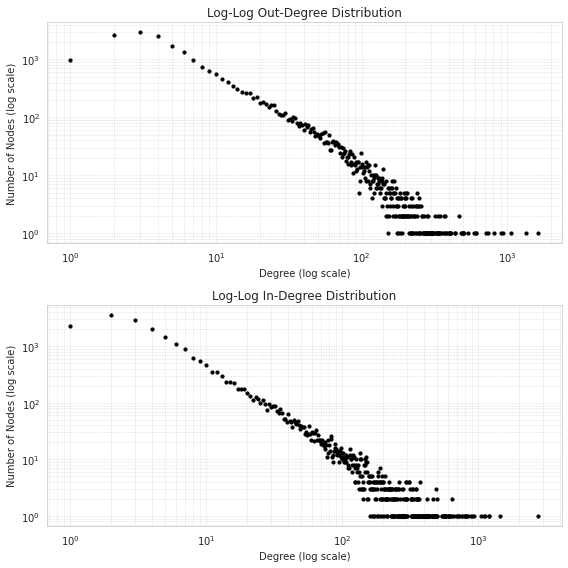
\includegraphics[width=0.4\textwidth]{img/loglog_core.png}}
    \centering
    \caption{log-log degree distribution for both out- and in-degree for the core subset}
    \label{fig:log_core}
\end{figure}

The straight line power-law distributions for both datasets indicate a scale-free network, which is common for social networks. The lower frequency of low degree nodes in the subset graphs show the removal of low degree nodes that are still present in the full dataset. The two graphs also show that the number of nodes with high-in degrees decreases at a lower rate than the number of nodes with high out-degrees. This suggests that a few influential nodes are highly trusted by many others, while most nodes only trust a small number of others. 

\subsection{Hub Analysis}
The tables below show the top 10 nodes by in-degree and out-degree for both the full dataset and subset. These important nodes are also called hubs. 

\begin{table}[h!]
\centering
\begin{tabular}{|c|c|c|}
\toprule
\textbf{Node} & \textbf{In-Degree} & \textbf{Out-Degree} \\
\midrule
\textbf{18} & 3,035 &  44 \\
\textbf{143} & 1,521 & 171 \\
\textbf{737} & 1,317 & 372 \\
\textbf{790} & 1,284 & 102 \\
\textbf{136} & 1,180 & 111 \\
\textbf{1,179} & 1,166 & 85 \\
\textbf{1,719} & 1,140 & 46 \\
\textbf{118} & 1004 & 123 \\
\textbf{4,416} & 941 & 106 \\
\textbf{780} & 908 & 3\\
\bottomrule
\end{tabular}
\caption{Top 10 node by in-degree.}
\label{tab:top_in_deg}
\end{table}

\begin{table}[h!]
\centering
\begin{tabular}{|c|c|c|}
\toprule
\textbf{Node} & \textbf{In-Degree} & \textbf{Out-Degree} \\
\midrule
\textbf{645} & 408 &  1,801 \\
\textbf{736} & 293 & 1,669 \\
\textbf{634} & 378 & 1,621 \\
\textbf{71,399} & 116 & 1,128 \\
\textbf{3,924} & 92 & 976 \\
\textbf{5,232} & 86 & 952 \\
\textbf{44} & 672 & 843 \\
\textbf{637} & 268 & 834 \\
\textbf{1,059} & 71 & 761 \\
\textbf{145} & 75 & 662\\
\bottomrule
\end{tabular}
\caption{Top 10 node by out-degree.}
\label{tab:top_out_deg}
\end{table}

The top node by in-degree (node 18) has an exceptionally high in-degree of 3035, indicating it is trusted by a large number of other nodes, while its out-degree (44) is relatively small. This trend suggests that highly trusted nodes do not necessarily reciprocate trust proportionately. About out-degree, node 645 leads the list with 1801 outgoing edges, indicating it trusts many other nodes, even though its in-degree (408) is comparatively lower. This implies a pattern of nodes that exhibit outgoing trust significantly more than receiving trust. By setting a threshold value of 600 for both the in-degree and the out-degree, the analysis identifies nodes with both in-degree and out-degree exceeding this threshold: only one node (44) meets this criterion, with an in-degree of 672 and an out-degree of 843, so this indicates that it is both highly trusted and highly trusting, which could signify a central or influential node in the trust network. After this study, it can be easily said that the network has clear asymmetry in trust relationships, where nodes with high in-degree are not necessarily those with high out-degree, and vice versa. Highly influential or central nodes (like node 44) with both high in-degree and out-degree are rare, suggesting that the trust network may have a hub-like structure with distinct roles for nodes. So, this analysis highlights the existence of "hubs" (nodes with high in-degree or out-degree), reflecting the heterogeneous nature of the trust dynamics in the network.
Considering the nodes with the highest in-degree value (hubs), 18 and 143, we will check whether they are directly connected. They are not, but only one node separates them (node 128). They are still part of the same connected component and have a relatively short path linking them. There are 588 nodes with outgoing edges to both 18 and 143, which is a significant number. These nodes serve as common predecessors, trusting both hubs simultaneously. This could indicate that nodes in the network often establish trust with highly influential or well-connected individuals.The common predecessors might represent users who trust multiple influential figures, potentially acting as bridges between communities.


\subsubsection{Ego Graph}
An ego-graph represents the subgraph centered on a specific node (called the "ego" node) and includes all nodes directly connected to it (neighbors) within a given radius. It is interesting to do this, for example, for node 18, and compare the relative graphs when node 18 is the top node for the in-degree in the core graph and when instead it is the top for out degree, as in the case of the reverse graph.

\begin{figure}[H]
    \centerline{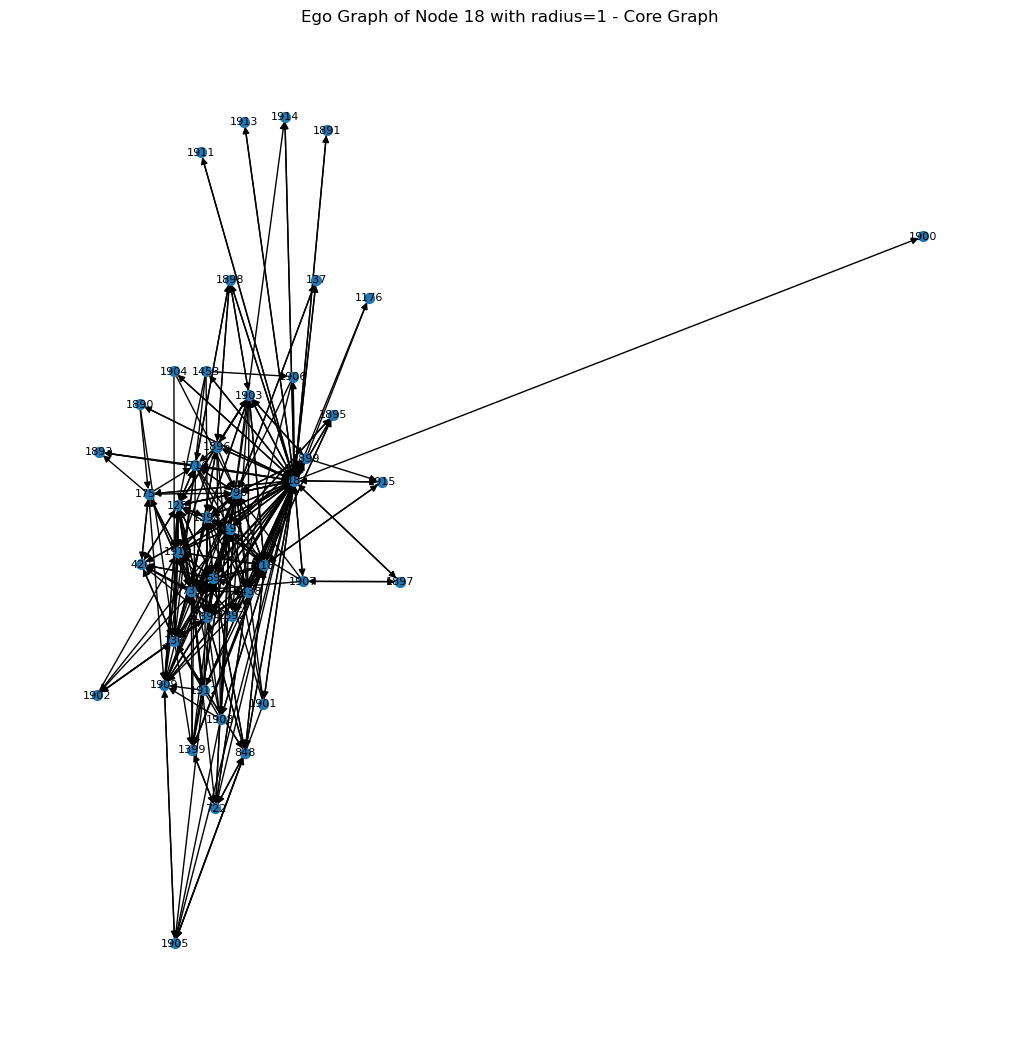
\includegraphics[width=0.4\textwidth]{img/node18_core.png}}
    \centering
    \caption{Ego graph of node 18 with radius = 1 - core graph}
    \label{fig:ego18core}
\end{figure}

\begin{figure}[H]
    \centerline{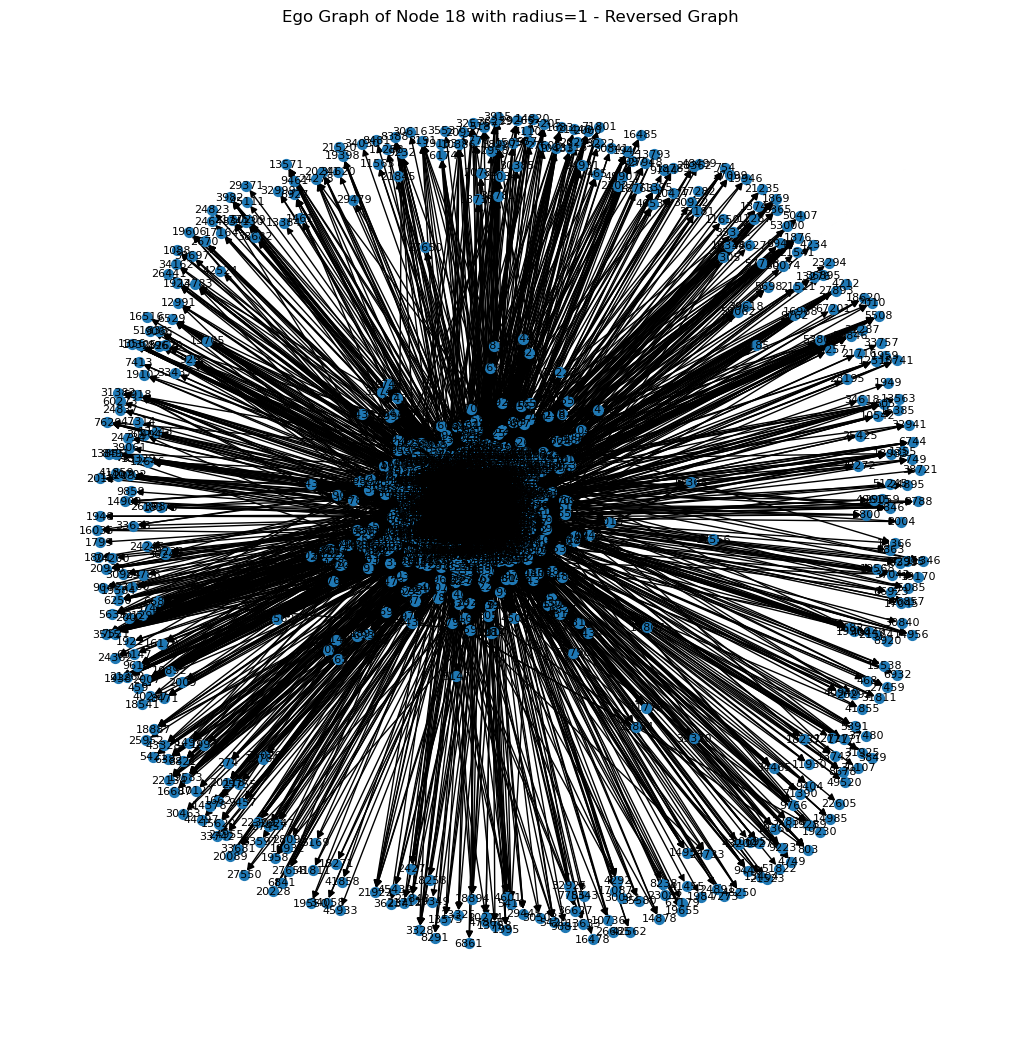
\includegraphics[width=0.4\textwidth]{img/node18_reversed.png}}
    \centering
    \caption{Ego graph of node 18 with radius = 1 - reversed graph}
    \label{fig:ego18core}
\end{figure}

The first plot represents the ego-graph of node 18 in the non-reversed graph. The edges represent trust relationships where node 18 is involved as the source or destination.It shows the direct "outgoing" and "incoming" connections around that node and arrows indicate who the node 18 trusts (outgoing edges) and who trusts node 18 (incoming edges). About the structure, dense clusters suggest that Node 18 is part of a highly interconnected group, nodes farther away or sparsely connected might represent weak or isolated trust relationships.
Instead, the second plot represents the ego-graph of node 18 in the reversed graph. The direction of all edges in the original graph has been flipped. In this context, it shows who trusts Node 18 in the reversed graph (where edges that were outgoing in the original graph become incoming, and vice versa). About differences, the plot seems to have a much larger spread of connections, suggesting that node 18 is trusted by many other nodes in the reversed graph.

\subsection{Degree Centrality}
The table below shows the top 10 nodes by degree centrality.

\begin{table}[h!]
\centering
\begin{tabular}{|c|c|c|c|}
\toprule
\textbf{\makecell{Node\\Full Dataset}} & \textbf{\makecell{Degree Centrality\\Full Dataset}} & \textbf{\makecell{Node\\Core Graph}} & \textbf{\makecell{Degree Centrality\\Core Graph}}\\
\midrule
\textbf{18} & 0.04058 &  18 & 0.11935 \\
\textbf{645} & 0.02911 & 645 & 0.08603 \\
\textbf{634} & 0.02634 & 634 & 0.07237 \\
\textbf{763} & 0.02585 & 143 & 0.06727 \\
\textbf{143} & 0.02229 & 737 & 0.06677 \\
\textbf{737} & 0.02225 & 44 & 0.06105 \\
\textbf{44} & 0.01996 & 736 & 0.05548 \\
\textbf{790} & 0.01826 & 34 & 05514 \\
\textbf{34} & 0.01730 & 790 & 0.05510 \\
\textbf{136} & 0.01701 & 136 & 0.05135 \\
\bottomrule
\end{tabular}
\caption{Top 10 nodes by degree centrality.}
\label{tab:top_deg_centrality}
\end{table}

\subsubsection{Degree Centrality of the Full Dataset}
The node 18, with a degree centrality of approximately 0.041, is the most connected node relative to the network size, reinforcing its role as a primary trust receiver. Other highly ranked nodes, such as node 645, also display strong connectivity, reflecting their roles as significant trust distributors. Nodes with high degree centrality are potentially influential or important in the network due to their large number of direct connections.

\subsubsection{Degree Centrality of the Core Graph}
The node 18, like for the original graph, has the highest degree centrality, but this measure now is bigger, indicating it is directly connected to roughly 11.9\% of the nodes in the graph. The degree centrality values decrease gradually, reflecting that other nodes like 645 and 634 also have significant but slightly lower direct connectivity within the graph.

\subsubsection{Mean Degree Centrality}
The mean degree centrality of the full dataset is 0.000177 and the mean degree  centrality of the core dataset is 0.00156. In our network, the mean degree centrality of the full dataset reflects a very sparse structure where most customers trust only a tiny fraction of the total population. The higher mean degree centrality in the core dataset indicates that the core network focuses on a smaller, denser group of individuals who are more interconnected and central to the trust structure.

\subsection{Detailed analysis core subset}
\subsubsection{Community detection by Louvain}
The results of running the Louvain algorithm on the full dataset and core subset are shown in table below. 

\begin{table}[h!]
\centering
\begin{tabular}{|c|c|c|}
\toprule
\textbf{Dataset} & \textbf{Full Dataset} & \textbf{Core Subset}\\
\midrule
\textbf{Number of communities} & 1,151 &  172 \\
\textbf{Level of modularity stabilization} & 7 & 5 \\
\textbf{Final modularity} & 0.533 & 0.412 \\
\bottomrule
\end{tabular}
\caption{Louvain Community Summary.}
\label{tab:louvain_community}
\end{table}

The number of communities is significantly larger in the subset than in the full dataset. This could be explained by the fact that the full dataset contains a significantly higher number of loosely connected nodes with a low degree, which can lead to a higher number of smaller communities. The algorithm took 2 more phases to obtain a stabilized modularity for the larger network, which is most likely due to the larger size of the full dataset. The table also shows that the final modularity is higher in the full dataset than in the core subset, meaning that the full dataset has better defined communities. The subset is likely denser, with a stronger connection among its nodes and less well-defined communities due to low degrees. Both modularity values indicate medium modularity, meaning that the network has a community structure but that communities could be more well defined and there is still a medium density of intertrust relationships.
 
The graphs below show the distribution of the nodes over the largest 10 communities for both the full dataset and subset. For the full dataset, 75\% of the nodes are in the 10 largest communities and for the subset 92\% of the nodes are in the 10 largest communities. This confirms the ideas that were discussed above. 

\begin{figure}[H]
    \centerline{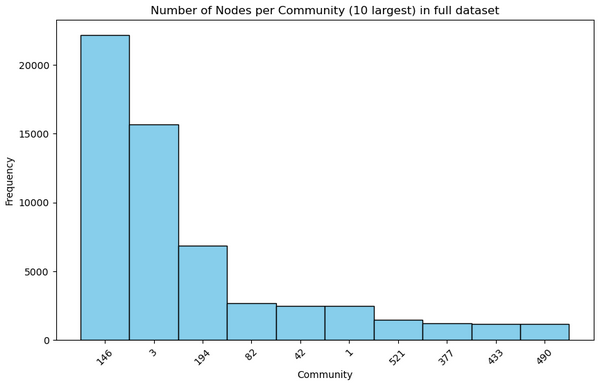
\includegraphics[width=0.4\textwidth]{img/louvain_network.png}}
    \centering
    \caption{Number of nodes per community (10 largest) in full dataset}
    \label{fig:ego18core}
\end{figure}

\begin{figure}[H]
    \centerline{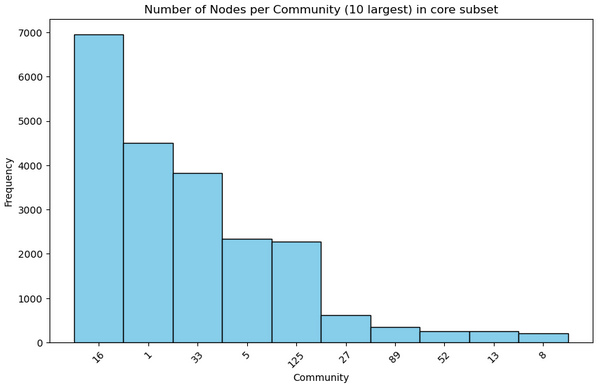
\includegraphics[width=0.4\textwidth]{img/louvain_core.png}}
    \centering
    \caption{Number of nodes per community (10 largest) in core subset}
    \label{fig:ego18core}
\end{figure}

The community size distribution graphs show that for the full subset, the largest community contains almost one third of the nodes, the second community about one fifth. For the subset this is similar. For the subset however, the third, fourth and fifth community are more significant in size compared to the two largest communities than for the full subset.

\paragraph{Hubs in subset communities}
The table below shows the communities that the hubs (the 10 nodes with the most in-degrees) of the core belong to. 

\begin{table}[h!]
\centering
\begin{tabular}{|c|c|c|c|}
\toprule
\textbf{Node} & \textbf{In Degree} & \textbf{Out Degree} & \textbf{Community}\\
\midrule
\textbf{18} & 3,035 &  44 & 44 \\
\textbf{143} & 1,521 & 171 & 33 \\
\textbf{737} & 1,317 & 372 & 1 \\
\textbf{790} & 1,284 & 102 & 16 \\
\textbf{136} & 1,180 & 111 & 33 \\
\textbf{1,179} & 1,166 & 85 & 33 \\
\textbf{1,719} & 1,140 & 46 & 16 \\
\textbf{118} & 1,004 & 123 & 33 \\
\textbf{4,416} & 941 & 106 & 33 \\
\textbf{780} & 903 & 3 & 33 \\
\bottomrule
\end{tabular}
\caption{Top 10 nodes by in-degree of the core and their community.}
\label{tab:top_in_deg_community}
\end{table}

The table above shows that most of the 10 largest nodes are in community 33, which is interesting, as it is not the largest community. Only node 790 with an in-degree of 1284 and node 1719 with an in-degree of 1140 are in the largest community of the core. The only hub from the top 10 that is in community 1, the second largest community, is hub 737 with an in-degree of 1317. None of the 10 largest hubs are in the other communities, which are all smaller than 2500 nodes.

\subsubsection{Spectral Clustering }
The eigenvalues and eigenvectors of the Laplacian were calculated, sorted and then analyzed to analyze the graph's structural properties.

\begin{figure}[H]
    \centerline{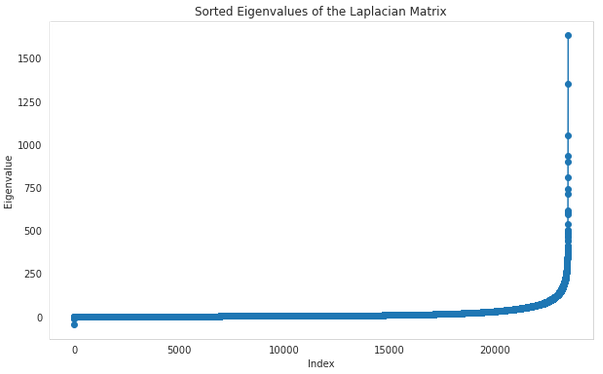
\includegraphics[width=0.4\textwidth]{img/sorted_eigenvalues_plot.png}}
    \centering
    \caption{Sorted Eigenvalues of the Laplacian Matrix}
    \label{fig:sorted_eigenvalues}
\end{figure}

The second smallest eigenvector (Fiedler vector) shows values clustered around zero, indicating that most nodes are part of a single dominant structure. A few outliers suggest substructures within the graph. 

\begin{figure}[H]
    \centerline{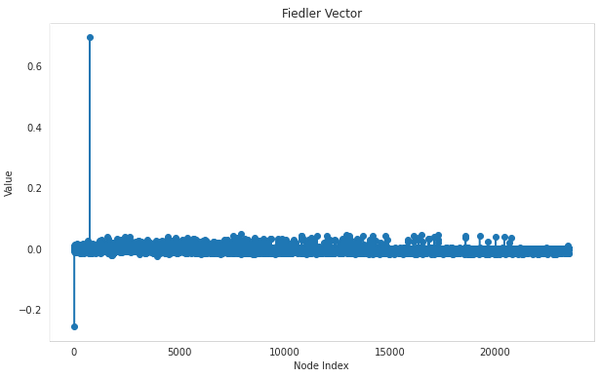
\includegraphics[width=0.4\textwidth]{img/fiedler_vector_plot.png}}
    \centering
    \caption{Fiedler Vector Plot}
    \label{fig:fiedler_vector}
\end{figure}

A spectral gap analysis was performed on the eigenvalues (as shown in the Spectral Gap Analysis plot). Based on the significant gaps, k=9 was selected as the number of clusters (one big gap close to 0, 8 big gaps close to 23000 on x axis).

\begin{figure}[H]
    \centerline{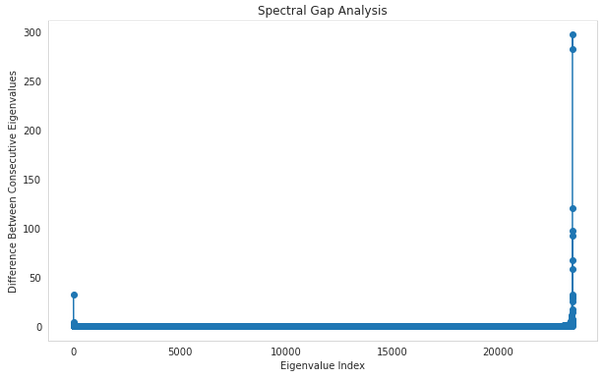
\includegraphics[width=0.4\textwidth]{img/spectral_gap_analysis.png}}
    \centering
    \caption{Spectral Gap Analysis}
    \label{fig:spectral_gap}
\end{figure}

The k-means algorithm was applied to the eigenvectors corresponding to the smallest 9 eigenvalues (excluding the first, which corresponds to the trivial zero eigenvalue).

\begin{itemize}
    \item The resulting clusters were analyzed for size, density (the ratio of edges within a cluster to the possible maximum), and modularity contribution (the degree to which the cluster contributes to the graph's modularity).
    \item The majority of nodes are assigned to Cluster 0, with a few much smaller clusters. This indicates a highly imbalanced clustering result, suggesting a dominant central structure in the graph and sparse outlying components.
\end{itemize}

\begin{figure}[H]
    \centerline{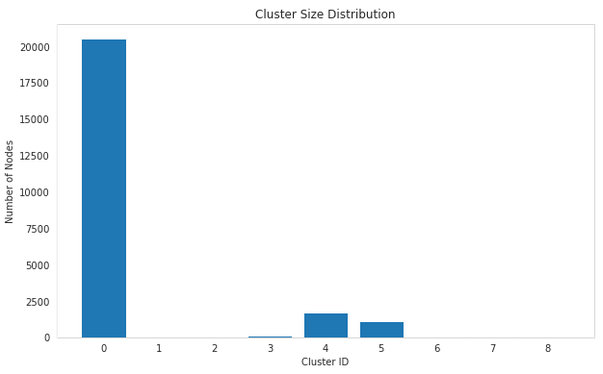
\includegraphics[width=0.4\textwidth]{img/9_cluster_size_distribution.png}}
    \centering
    \caption{Cluster Size Distribution - 9 clusters}
    \label{fig:cluster_size_dist_9}
\end{figure}

Here is a summary of key properties for each cluster:

\begin{table}[h!]
\centering
\begin{tabular}{|c|c|c|c|c|}
\toprule
\textbf{Cluster ID} & \textbf{Nodes} & \textbf{Edges} & \textbf{Density} & \textbf{\makecell{Modularity\\Contribution}}\\
\midrule
\textbf{0} & 20,519 &  311,608 & 0.0007 & -0.0402 \\
\textbf{1} & 1 & 0 & 0.0000 & 0.0000 \\
\textbf{2} & 1 & 0 & 0.0000 & 0.0000 \\
\textbf{3} & 106 & 547 & 0.0491 & 0.0012 \\
\textbf{4} & 1,689 & 0.0073 & 0.0429 \\
\textbf{5} & 1,130 & 1,504 & 0.0012 & 0.0012 \\
\textbf{6} & 1 & 0 & 0.0000 & 0.0000 \\
\textbf{7} & 55 & 70 & 0.0236 & 0.0002 \\
\textbf{8} & 1 & 0 & 0.0000 & 0.0000 \\
\bottomrule
\end{tabular}
\caption{9-cluster summary.}
\label{tab:9_cluster_sum}
\end{table}

Where:
\begin{itemize}
    \item The lower density indicates the loose connection, suggesting the less cohesivity, while the higher density indicates tighter connections within this group, showing a cohesive substructure 
    \item The negative modularity contribution suggests it does not strongly contribute to graph modularity, while the higher density shows that the cluster is a well-defined community.
    \item The community without edges indicates isolated nodes without contribution to modularity.    
\end{itemize}

\begin{figure}[H]
    \centerline{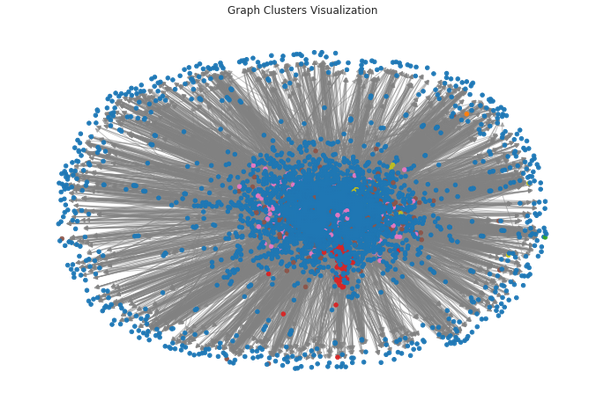
\includegraphics[width=0.4\textwidth]{img/graph_9_cluster_visualization.png}}
    \centering
    \caption{Plot of the graph with nodes colored by their cluster - 9 cluster}
    \label{fig:9_cluster_graph_plot}
\end{figure}

Due the presence of isolated cluster, let’s try to reduce the number of clusters from 9 to 5:

\begin{table}[h!]
\centering
\begin{tabular}{|c|c|c|c|c|}
\toprule
\textbf{Cluster ID} & \textbf{Nodes} & \textbf{Edges} & \textbf{Density} & \textbf{\makecell{Modularity\\Contribution}}\\
\midrule
\textbf{0} & 1,584 &  15,378 & 0.0061 & 0.0311 \\
\textbf{1} & 17,364 & 89,135 & 0.0003 & -0.3393 \\
\textbf{2} & 1,093 & 1,405 & 0.0012 & 0.0011 \\
\textbf{3} & 1 & 0 & 0.0000 & 0.0000 \\
\textbf{4} & 3,461 & 156,360 & 0.0131 & 0.3406 \\
\bottomrule
\end{tabular}
\caption{5-cluster summary.}
\label{tab:5_cluster_sum}
\end{table}

\begin{figure}[H]
    \centerline{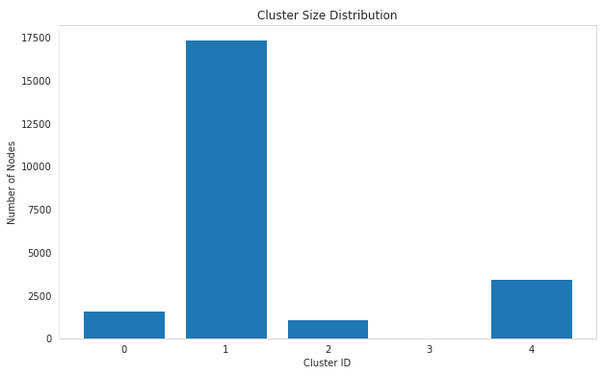
\includegraphics[width=0.4\textwidth]{img/5_cluster_size_distribution.png}}
    \centering
    \caption{Cluster Size Distribution - 5 clusters}
    \label{fig:cluster_size_dist_5}
\end{figure}

\begin{figure}[H]
    \centerline{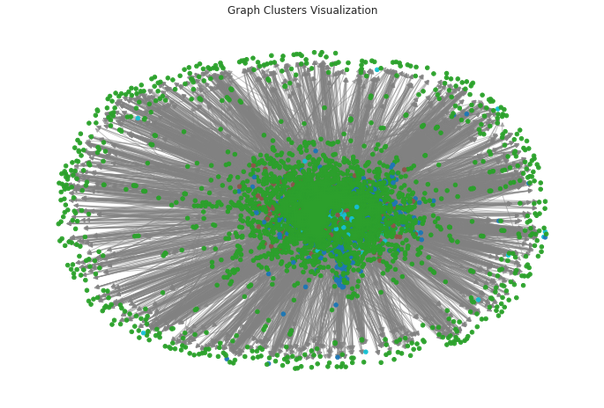
\includegraphics[width=0.4\textwidth]{img/graph_5_cluster_visualization.png}}
    \centering
    \caption{Plot of the graph with nodes colored by their cluster - 5 cluster}
    \label{fig:5_cluster_graph_plot}
\end{figure}

Trying to further reduce the number of clusters, we always get a cluster with one single node, indicating the presence of one isolated element, really far from the others.

\subsubsection{Simulation of Opinion Dynamics}
By running the simulation, we observed the influence spread rapidly, with a large initial wave of nodes transitioning to "awake." Most nodes adopted the "awake" state within 25 steps, indicating a fast convergence driven by the hubs. A sharp decline in the number of state changes was observed after the first few steps, reflecting rapid stabilization.
Hubs in the original trust graph played a critical role in spreading opinions. Their initialization as "awake" nodes created a cascade effect, influencing the majority of the network. Reversing the graph direction effectively modeled how trusted nodes (hubs) propagate their opinions to those who trust them, aligning with the goal of analyzing opinion influence.

\paragraph{Implications}
In real-world systems (e.g., social media or reputation systems), highly trusted individuals can have an outsized impact on opinion dynamics. Interventions targeting such nodes may efficiently shape overall network behavior.
The sharp decline in state changes after initial steps suggests that early intervention (e.g., seeding influential nodes with opinions) can rapidly propagate influence.

\paragraph{Visualizations}
\begin{figure}[H]
    \centerline{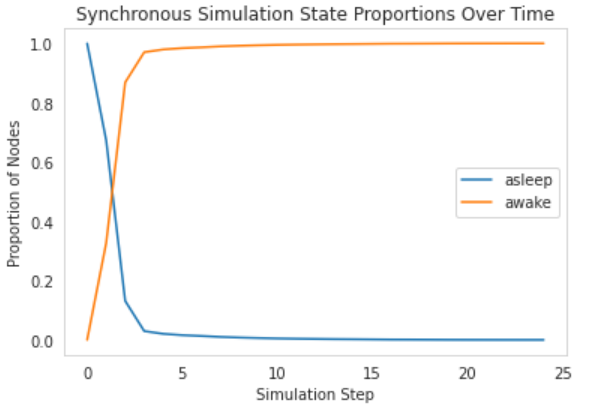
\includegraphics[width=0.4\textwidth]{img/simulation_proportions.png}}
    \centering
    \caption{Simulation State Proportion Over Time}
    \label{fig:sim_prop}
\end{figure}
\begin{figure}[H]
    \centerline{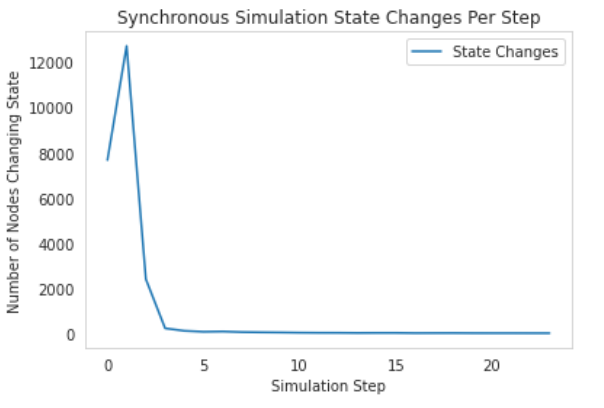
\includegraphics[width=0.4\textwidth]{img/simulation_changes.png}}
    \centering
    \caption{Simulation State Changes Per Step}
    \label{fig:sim_changes}
\end{figure}

\section{Discussion and conclusion}
This study analyzed the "soc-Epinions1" dataset to uncover insights into trust dynamics and the structural properties of an online social network. The analysis of the full dataset and the core subset provided us with several findings. The core network revealed a denser and more interconnected structure compared to the full dataset. This highlights that trust relationships are often concentrated among a smaller group of active and influential participants. Real-world applications, such as reputation systems and targeted marketing campaigns, could leverage such insights by focusing on highly connected users to optimize impact. 

The analysis of hub nodes underscored the asymmetric nature of online trust relationships. For instance, certain nodes were highly trusted but did not trust others at the same level. The network moreover showed scale-free characteristics, with few nodes having disproportionately high connections. Organizations can use such properties to design efficient information dissemination strategies.

Through the Louvain analysis, communities for both the full dataset and the subset with a medium modularity were found, with a value that was slightly higher for the full dataset than for the subset. The Louvain analysis showed that for the full dataset 75\% of the nodes were in the 10 largest communities and for the subset 90\% of the nodes were in the 10 largest communities. This confirms the idea described above. The 10 largest hubs of the subset were divided over 3 different communicates. This indicates that there are different important influential cores of trust within the subset. Surprisingly, only 2 of the 10 largest hubs were found in the largest community of the core graph, which had about one third of all the nodes and most of the 10 largest hubs were found in the third largest community. This means that the largest community might not be as important as its size suggests and that the cohesion is lower there. The communities that were found in this study using Louvain could indicate  users of similar interest (interest in the same products), similar standards of judgment, or geographic location. 

For the spectral clustering, it was found that 5 is the ideal number of clusters, which is a much lower number than the 171 communities found by the Louvain algorithm. According to the k-means analysis, the network’s structure is dominated by a central cluster, which has more loosely connected nodes. Smaller clusters represent tightly connected communities with significant positive modularity contributions. 

Finally, talking about the simulation, it showed that influential nodes (hubs) play an important role in propagating opinions across the network, since rapid adoption of ideas was observed. This suggests that early intervention or strategic seeding of ideas through key influencers can achieve widespread adoption in a short time. This finding is particularly relevant for designing campaigns in social media and behavioral change initiatives.

The insights gained from this study have broader implications for real-world systems. For example, for social media, streaming platforms or e-commerce trust-based algorithms could enhance content visibility by prioritizing reviews or posts from highly trusted users. In addition, it can be used for public policy and education, since understanding how information spreads can guide strategies to address societal challenges like misinformation or polarization. Further studies could for example dive deeper into how implicit and indirect trust can be deduced from who-trusts-whom networks, about how trust relationships can influence opinions formation and trust relationships between different communities. 


\printbibliography 

\end{document}